% !TeX root = ../thesis.tex
% !TeX spellcheck = en_US

In this chapter, basic concepts are described, which are relevant for this thesis.
Primarily, this includes geodata, routing algorithms as well as agent-based simulations.
The section about geodata gives a broad overview of coordinate systems, file formats, standards and OpenStreetMap, which is the geodata source in this thesis.
Geodata can generally be used to find the shortest paths between two locations using routing algorithms.
Two main strategies exist to find such paths, graph-based and geometric routing, and both will be covered in this chapter.
Agent-based simulations play an essential role in pedestrian simulations and often use these routing algorithms for the agent's movements.
Hence, the topic of agents and simulations will be covered as well.

\section{Geospatial data}

	According to the ISO standard 19109:2015\cite{iso-19109}, the term \term{geospatial data} refers to \enquote{data with implicit or explicit reference to a location relative to the Earth}.
	In other words, data with an address, coordinate or any other kind of location reference belongs to the class of \term{geospatial data}, or \term{geodata} for short.
	
	Examples are customer information (address information of each customer), meteorological data (measured temperature and humidity with a coordinate and altitude) and, primarily used in this thesis, road and path data suitable for routing.
	Addresses are less important for this thesis, as they are not globally standardized, only describe a vague location and usually belong to a whole area.
	Geodata may have an additional time dimension and is therefore categorized as \term{spatiotemporal data}\cite{iso-19108}.
	Even though the time dimension is relevant in many real-world use cases, this type of data is of less importance for this thesis as well.
	This thesis uses the term \emph{geodata} to refer to data structures described below in \Cref{subsec:data-structures}.
	
	Besides the mentioned explicit references to locations, such as coordinates, implicit location references can also be encoded within the metadata of datasets.
	One example is the image-based GeoTIFF format described in \Cref{subsubsec:geotiff-format}.
		
	\subsection{Data structures}
	\label{subsec:data-structures}
	
		Spatial data can be stored in a variety of data structures.
		Some are used in many frameworks, libraries and formats, but some are vendor specific.
		An overview of common data structures in spatial data is given in this section.
		
		The \term{Simple Feature Access} (\term*{SFA}) standard by the Open Geospatial Consortium (\term*{OGC}) defines numerous geometry types\cite{ogc-sfa}.
		Not all of them are implemented in all data formats, and most are irrelevant for this thesis.
		The \term*{GeoJSON} file format (described in more detail in \Cref{subsubsec:geojson}) implements the most important geometries and data structures of the SFA standard and is frequently used in this work.
		This section gives an overview of these geometry types and an introduction to the concept of features.
		
		\subsubsection{Geometries}
		
			A \term{geometry} only represents geometric coordinates and their relation to each other.
			Common types of geometries are:
			\begin{description}
				\item[Point] Simple geometry type with only one coordinate.
				\item[LineString] An ordered list of multiple coordinates building a line with a certain direction.
				\item[Polygon] An ordered list of coordinates of which the first and last coordinates are equal and thus form an area. A polygon might consist of additional polygons inside of it, forming holes. Polygons inside such holes form islands, which can have holes again.
				\item[Multi-Geometries] Grouping geometries of the same type together forms multi-geometries, such as \texttt{MultiPoint}, \texttt{MultiLineString} and \texttt{MultiPolygon}. They can be used to share properties of the contained geometries.
			\end{description}
		
		\subsubsection{Features}
		
			A \term{feature} is an abstraction of a world phenomenon, for example, a tree, road or lake.
			From a technical perspective, a feature consists of a geometry, describing \textit{where} the feature is, and attributes (also called \enquote{properties} or \enquote{tags}), describing \textit{what} the feature represents.
			Different file formats have different properties regarding geometries and attributes, which will be described in the following sections.
		
		\subsubsection{Standardization}
		
			Standards exist to keep a data source consistent and allow system interoperability.
			Common standards were defined by organizations like the OGC as well as companies or government agencies.
			
			A widely used proprietary standard established by Esri Inc. is the Shapefile file format, which will be covered in \Cref{subsubsec:other-formats}.
			One example of a governmental standard is the \term{INSPIRE} standard based on an initiative of the European Commission\footnote{\url{https://inspire.ec.europa.eu}}.
			Next to proprietary or governmental standardizations, the \term*{OpenStreetMap} project uses a system based on proposals and democratic votes, which is further described in \Cref{subsec:osm}.
			
		\subsection{Spatial indices}
		
			Storing data for efficient access, e.g. to query all features within a particular area, a so-called \term{spatial index} is used.
			Some commonly used indices are the following.
			
			The \term[k-d tree]{$k$-d tree}\cite[Ch.\ 19,p. 4]{mehta-handbook-data-structures} divides the space at each vertex along one axis at a time alternating through all axis (dimensions) of the dataset, which leads to a binary tree for 2-dimensional data.
			A \term{quadtree}\cite[Ch.\ 19,p. 1]{mehta-handbook-data-structures} works on 2-d data and divides the space equally into four equally sized quadrants.
			Depending on the data in each quadrant, it gets divided again, which leads to a tree with four children per node.
			The \term{R-tree}\cite[Ch.\ 21,p. 2]{mehta-handbook-data-structures} determined bounding rectangles for areas with dense data and efficiently stores a hierarchy of these areas, i.e. all features of child nodes are within the bounding rectangle of the parent node.
			
			In the implementation of the hybrid routing algorithm, some of these indices are used to enhance performance, as presented and analyzed in the later chapters of this work.
			
	\subsection{File formats}
	\label{subsec:file-formats}
	
		Spatial data can be stored in various file formats with different properties and use cases.
		This section gives an overview of some popular formats.
		
		\subsubsection{GeoJSON}
		\label{subsubsec:geojson}
		
			Another open but not OGC-standardized format is \term{GeoJSON}, which is the most important format for this thesis as all used datasets were in this file format.
			As the name suggests, a GeoJSON file follows the JSON specification defined in RFC7946\footnote{\url{https://datatracker.ietf.org/doc/html/rfc7946}}.
			The file can either contain a collection of features (of type \texttt{FeatureCollection}) or geometries (of type \texttt{GeometryCollection}, which itself is a geometry type).
			Each feature in a \texttt{FeatureCollection} consists of a geometry and, in contrast to elements in a \texttt{GeometryCollection}, attributes adding additional information to the feature.
			The number of geometries per feature as well as their length, number and character choice of attributes is not restricted.
			
		\subsubsection{GeoTIFF}
		\label{subsubsec:geotiff-format}
		
			All formats mentioned so far store vector data, but raster data can also be georeferenced.
			One image-based format to store such raster data is the OGC-standardized \term{GeoTIFF} format\cite{ogc-geotiff}, which is a TIFF formatted image with spatial metadata such as the coordinate system and a mapping of pixel to coordinates.
			Typical use cases for such images are aerial or satellite imagery and \term*[digital elevation model]{digital elevation models} (\term*{DEM}).
			However, other use cases are thinkable, such as field-based routing algorithms as mentioned in \Cref{subsec:field-based-routing} using raster data to store the vector fields.
		
		\subsubsection{Other formats}
		\label{subsubsec:other-formats}
		
			Other formats are for example \term{Well-known Text} (\term*{WKT}), consisting of the geometry type followed by a list of coordinates\cite[51]{ogc-sfa}, \term{GeoPackage}\footnote{\url{http://www.geopackage.org}}, consisting of a SQLite database with support for spatial functions and indices, or the widely used and proprietary \term{Esri Shapefile} format\cite{esri-shapefile-spec}.
			However, numerous additional formats exist for general and special use cases.
			
	\subsection{OGC web services}
	
		Besides file-based formats, web-based standards exist as well.
		The OGC standardized some APIs for web-based services.
		Popular standards are the \term{Web Map Service} (\term*{WMS}), \term{Web Map Tile Service} (\term*{WMTS}) and \term{Web Feature Service} (\term*{WFS}).
		These services are only used to interact with the raw data but do not offer higher-level functionalities such as routing.
	
	\subsection{GIS}
	
		A file format alone, as described in \Cref{subsec:file-formats}, is only useful when storing or transferring data and to ensure interoperability.
		Processing the data is part of applications referred to as \term[geographic information system]{geographic information systems} (\term*{GIS}).
		
		The term GIS is very broad and describes nearly all systems working with spatial data.
		This includes databases like Postgres with the PostGIS extension, software libraries like the \term*{NetTopologySuite}, servers like \term*{GeoServer} and desktop applications like \term*{ArcMap} or \term*{QGIS}.
		Such desktop applications often combine multiple functionalities to visualize, analyze or otherwise process the data.
	
	\subsection{OpenStreetMap}
	\label{subsec:osm}
	
		\term{OpenStreetMap} (\term*{OSM}) is a publicly available and freely accessible geospatial database that is maintained by a global community and licensed under the \emph{Open Data Commons Open Database License} (\term*{ODbL})\cite{osm-wiki-about}.
		It can therefore be used, changed and redistributed as long as proper attribution is given and results stay under the ODbL\footnote{\url{https://opendatacommons.org/licenses/odbl}}.
		All spatial data used in this thesis is data from the OSM database.
		In 2006, two years after the OSM project started, the OpenStreetMap Foundation\footnote{\url{https://osmfoundation.org}} was established to perform fund-raising, maintain the servers and also act as a legal entity for the project.
		People contributing to OSM are called \textit{mappers} or \textit{contributors}, often working voluntarily and mapping their local vicinity or concentrating on specific topics.
		
		\subsubsection{Data model}
		
			The model of OSM is much simpler compared to many of the \hyperref[subsec:file-formats]{aforementioned} data formats.
			There are three main data types in OSM: \term{node}, \term{way} and \term[relation]{relations}\cite{osm-wiki-data-model}.
			
			Nodes and ways are analogous to \texttt{Point} and \texttt{LineString} from the OGC \term*{Simple Feature Access} (\term*{SFA}) specification described in \Cref{subsec:data-structures}.
			Areas also exist but are modeled as closed ways and therefore do not form a new type of geometry.
			A way is closed when the first and last coordinates are identical and specific area-compatible attributes are set.
			
			Relations form a collection of features, so they correspond to \texttt{MultiPoint}, \texttt{MultiLineString} and \texttt{MultiPolygon} of the SFA specification.
			Typical use cases are multipolygons, road segments involved in turn restrictions and ways included in a bus route.
			
		\subsubsection{Attributes}
		\label{subsubsec:osm-attributes}
			
			Attributes are called \term[tag]{tags} in OSM, are simple unrestricted key-value pairs and mostly describe properties of features.
			For example, a restaurant (\texttt{amenity=restaurant}) may have additional tags such as the name, address and opening hours.
			
			Some tags, like \texttt{area=[yes|no]} or the relation-specific \texttt{type}-key, influence the type of geometry.
			A closed way with \texttt{area=no} does, in fact, \textit{not} represent a polygon, but just a closed linestring.
			This not only affects visualizations but may also need to be considered in other processing and analysis tasks.
			Other tags add metadata to objects, for example, the last time the feature was surveyed, the source of the data or internal notes to other mappers.
			
			The OSM community organizes the standardization of tags in the project's wiki via a special proposal process\cite{osm-wiki-proposal-process}.
			To ensure flexibility, it is explicitly allowed to use new, reasonable and unstandardized tags, which may become de facto accepted if they are commonly used.
			Proposed tagging scheme changes to not only get accepted or rejected by a democratic vote, a mandatory public discussion of at least two weeks needs to take place prior to voting.
			Due to the vast amount of contributors, different opinions, use cases, editors and knowledge about the tagging schemes, multiple competing schemes evolved for some attributes (for example \texttt{phone=*} and \texttt{contact:phone=*}).
			Tagging schemes change over time and some may become deprecated or are officially abandoned via a proposal, which might lead to outdated tags on objects.
			
		\subsubsection{Contributions to OSM}
		
			Uploads to OSM always happen in so-called \term[changeset]{changesets} combining multiple changes on the map\cite{osm-wiki-changeset}.
			Like features, each changeset itself can contains tags adding metadata to the change.
			Tags like \texttt{created\_by} (containing the username), \texttt{comment} (describing the change) and \texttt{source} (data sources like aerial imagery or manual survey) are the most common ones but editors may add additional information.
			The \texttt{source} tag is particularly important since the ODbL is not necessarily compatible with licenses of other data sources and this tag helps to verify this compatibility.
			Ideally, a changeset should be coherent, which means that it should focus on one thematic aspect in one local area, but this is not always the case and some editors automatically split larger changesets into smaller ones.
			
		\subsubsection{Data contained in OSM}
		
			OSM has no focus on specific topics and nearly anything can be added to OSM due to the flexible tagging scheme.
			However, some types of features are very common according to \emph{taginfo}, an online service providing daily updated statistics on keys and values in OSM\footnote{\url{https://taginfo.openstreetmap.org/keys}}.
			According to these statistics, the most common objects are buildings with over 542 million occurrences.
			Furthermore, 6\% of all objects and nearly 60\% of all ways are buildings.
			Highways (mainly roads and streets but also paths, bridleways, railways and more) are the second most common features with over 219 million ways (23\% of all ways).
			Addresses are also very common: about 32\% of all nodes and 7\% of all ways (mainly building) have a house number.
			Other often added area features are forests and lakes as well as line features like barriers and waterways.
			
		\subsubsection{Data \textit{not} contained in OSM}
		\label{subsubsec:data-not-in-osm}
		
			Even though the tagging scheme can be extended arbitrarily, some data will probably not be added to OSM, which can have multiple reasons:
			
			\begin{itemize}
				\item Some data is too detailed and therefore mappers are unlikely to invest the time necessary to create or maintain that data.
				For example, features representing historic buildings are made of long straight lines even though the real building facade is detailed and richly designed.
				\item Data that cannot be verified on the ground will likely not be added to OSM, because anyone visiting the data in the real world should be able to verify its existence and correctness.
				\item Temporary data should not be added since OSM is not a real-time database.
				However, there is no strict definition of when a feature is temporary and when it is (potentially) permanent.
				\item Data under an incompatible license will not be added.
				This also includes data from many public authorities and nearly all companies.
				\item Private areas are often not part of OSM or contain only a few details.
				This is mainly because access to private areas is usually restricted, rendering them unverifiable for unauthorized mappers.
			\end{itemize}
			Unfortunately, data relevant to routing is often added to ways representing roads and paths but not to areas.
			This includes primarily accessibility and surface information.
			However, the latter can sometimes be inferred or approximated from other tags on a polygon, for example, \texttt{surface=grass} from \texttt{leisure=park}, but there is always the possibility for errors.
			
		\subsubsection{Data used in this thesis}
		
			This thesis uses OSM data for routing purposes.
			Other sources of spatial data exist but are non-free (in terms of price and the license of the data), fragmented over multiple sources (files, servers, APIs) or not as detailed as OSM.
			
			One example of such a fragmented source is provided by the state office for geoinformation and surveying (Landesbetrieb für Geoinformationen und Vermesseung -- LGV) in Hamburg, Germany.
			Many datasets can be downloaded from the official website \href{https://geoportal-hamburg.de}{geoportal-hamburg.de} but roads and building data are contained in separate datasets, primarily \enquote{HH-SIB} and \enquote{ALKIS}.
			In addition to the fragmentation, some of data is not suitable for routing.
			The \enquote{HH-SIB} dataset contains numerous line segments, which represent ways and roads, that are not connected to the remaining road network.
			The \enquote{ALKIS} dataset also contains road data, but only as areas, which is not suitable for routing as well.
			However, OpenStreetMap offers free access to numerous usable features in one dataset.
			
			Since geometric routing is the major topic, not only the road network is used, but also certain features of OSM representing impassable obstacles, which are avoided during routing:
			\begin{itemize}
				\item \textbf{Barriers}: The \texttt{barrier}-tags describe non-passable barriers but also passable structures like gates. Thus, only specific barriers (mainly fences and walls) are considered.
				\item \textbf{Buildings}: The \texttt{building} tag describes any type of building. However, values such as \texttt{building=roof}, \texttt{=no} and \texttt{=demolished} are not considered.
				\item \textbf{Natural areas}: Areas with the \texttt{natural}-key describe areas filled with a specific form of vegetation as well as water areas. All natural areas, except grass-covered land, are considered.
				\item \textbf{Railway}: Any type of railway infrastructure (\texttt{railway=*}) is considered.
				\item \textbf{Waterways}: All waterways, such as rivers, canals or ditches, are considered.
			\end{itemize}
			The exact choice of the passable and impassable features is debatable or depends on the simulation's domain.
			For example, train tracks might be passable in an evacuation scenario.
			
			The road network is also used, which is done by importing all features with a \texttt{highway} key.
			Features such as stop signs or streetlights, which are not part of the road network, are not removed because they may contain information useful for routing.

\section{Graph-based routing}
\label{sec:graph-routing}

	\subsection{Theoretic considerations}
	\label{subsec:routing-theoretic-considerations}	
	
		Routing refers to the process of finding the optimal (often shortest) path between two given locations.
		Graph-based routing takes place on a graph $G=(V, E)$ with $V$ being the set of vertices and $E \subseteq V \times V$ being the set of edges connecting the vertices\cite[643-644]{cormen-introduction-to-alg}.
		To goal is to find a path from a source $s \in V$ to a destination (or target) $t \in V$ of minimal weight using a weight function $w: E \rightarrow \mathbb{R}$.
		A path $p=\left\langle v_0, v_1, \dots v_n \right\rangle$ is an ordered list of connected vertices $v_0, v_1, \dots, v_n \in V$, which means for two consecutive vertices $v_i$ and $v_{i+1}$, $(v_i, v_{i+1}) \in E$ must hold.
		
		Often the shortest path is to be determined, which is why the weight function is used to calculate the length of an edge.
		Even though the following sections refer to shortest paths, determining \enquote{optimal} (or minimal) paths is the general case.
		Thus, routing is a minimization problem, trying to find a path $p$ of minimum weight $w(p) = \sum_i{w(v_i, v_{i+1})}$.
		
		In theoretic computer science, the fundamental problem behind routing algorithms is called the \term{shortest paths problem}, which exists in the following variants.
		
		\subsubsection{\term*[single-source shortest paths]{Single-source shortest paths}}
		\label{subsubsec:single-source-shortest-path}
		
			One source vertex is given and the shortest paths to all other vertices should be determined.
			Algorithms solving this problem are, for example, the Dijkstra algorithm, described in detail in \Cref{subsubsec:dijkstra}, or the Bellman-Ford algorithm, which can additionally handle negative edge weights\cite[651]{cormen-introduction-to-alg}.
		
		\subsubsection{\term*[single-destination shortest paths]{Single-destination shortest paths}}
		
			This is the opposite of the above problem.
			All shortest paths to a specific vertex from any other vertex should be found.
			However, no new algorithms are needed to solve this problem.
			Instead, the direction of each edge can be reversed, turning this problem into the single-source problem.
		
		\subsubsection{\term*[single-pair shortest paths]{Single-pair shortest paths}}
		
			The shortest path from one specific source to one specific destination vertex should be determined.
			Even though there are specialized algorithms for this problem like \term*{TRANSIT} (described in \Cref{subsubsec:other-speedup-methods}), more general approaches to solve the single-source problem can be used as well, such as the Dijkstra algorithm as presented in \Cref{subsubsec:dijkstra}.
		
		\subsubsection{\term*[all-pair shortest paths]{All-pair shortest paths}}
		\label{subsubsec:all-pair-shortest-path}
		
			This problem is similar to the single-source problem, but every vertex is a source vertex.
			A naive approach would likely use an algorithm to solve the single-source problem of each vertex.
			However, there are faster ways to solve this, such as the Floyd-Warshall and Johnson's algorithm\cite[693,700]{cormen-introduction-to-alg} as well as PHAST\cite{bast-transportation-networks} with a complexity of $\Theta(|V|^2)$.
		
	\subsection{Routing engines and shortest path algorithms}
	\label{subsec:routing-engines}
		
		The term \term{routing engine} refers to software built to find an optimal route between a source and destination location.
		The optimality of this route is determined by a routing profile, which is a weighting function assigning a weight to each edge in the input graph.
		Routing engines might perform other operations as well, such as the calculation of \term[isochrone]{isochrones}, which are a way to visualize the reachability of a region\cite{allen-isochrones}.
		Each isochrone is an area reachable from a given source location within the same amount of time, which is determined using routing.
		
		To find desirable paths, the weight function $w$ mentioned in \Cref{subsec:routing-theoretic-considerations} needs to be carefully chosen based on the domain of the application, vehicle type, personal preferences and other influencing factors.
		Navigation applications in everyday life bundle these aspects into a \term{routing profile}, which maps attributes from the input data to a certain weight.
		Input data might consist of multiple sources like a road network, a digital elevation model or additional traffic information.
		The open-source software \term*{GraphHopper} is one example of a routing engine and comes with predefined profiles for different modalities and situations.
		For example, the \texttt{car\_delivery} profile is made for car-based delivery services enabling the use of private roads\cite{graphhopper-routing-profiles}, which are avoided in the normal \texttt{car} profile.
		
		To enhance performance, speedup methods were developed, allowing routing queries of continental or even global sizes to be answered quickly.
		Some popular methods are, among others, \term{contraction hierarchies} and \term[landmark]{landmarks}, which will both be described with more details in \Cref{subsec:speedup-methods}.
		
		\subsubsection{Dijkstra}
		\label{subsubsec:dijkstra}
		
			Dijkstra's algorithm, often just called \term{Dijkstra}, is originated in the 1950s and can be used to solve the \term*{single-source shortest paths} problem.
			When no destination vertex is given, it creates a spanning tree rooted in the source vertex $s$ containing solely shortest paths to all other vertices.
			Despite its age, Dijkstra's algorithm and optimized versions of it are frequently used in science and real-world applications.
			\Cref{alg:dijkstra} presents an enhanced version using a priority queue for the vertices\cite[658]{cormen-introduction-to-alg}.
			
			\begin{algorithm}[h]
				\begin{algorithmic}[1]
					\ForAll{vertices $v \in V$}
						\State Set shortest path distance $v.d = \infty$ and predecessor vertex $v.\pi = undefined$
					\EndFor
					\State $s.d = 0$
					\State Insert all vertices into min-priority queue $Q$ with $v.d$ being the priority
					\State $S = \emptyset$
					\While{$Q \neq \emptyset$}
						\State Get closest vertex $u = Q.min$
						\ForAll{adjacent vertices $v$ of $u$}
							\State Add $u$ to $S$
							\If{the path to $v$ via $u$ is shorter than $v.d$, so if $u.d + d(u, v) < v.d$}
								\State Set $v.d = u.d + d(u, v)$ and $v.\pi = u$
							\EndIf
						\EndFor \label{alg:dijkstra:end-inner-loop}
					\EndWhile
				\end{algorithmic}
				\caption{Pseudocode of Dijkstra's algorithm using a priority queue and starting at vertex $s \in V$.}
				\label{alg:dijkstra}
			\end{algorithm}
			\noindent
			Once a vertex is taken from the queue, it is considered as \emph{visited} by adding it to $S$.
			It can be proven that for each visited vertex $v$, the distance $v.d$ after the last iteration of the inner for-loop is optimal\cite[659-661]{cormen-introduction-to-alg}.
			This also means following back the predecessor relation $v.\pi$ yields the shortest path.
			When $u$ is equal to a destination vertex $t$, the algorithm can safely be stopped after line \ref{alg:dijkstra:end-inner-loop} since the optimal path from $s$ to $t$ has been found.
		
		\subsubsection{A*}
		\label{subsubsec:astar}
		
			The \term{A*} shortest path algorithm was introduced in 1968 and uses a heuristic $h : V \rightarrow \mathbb{R}$ in combination with a distance function $g : V \rightarrow \mathbb{R}$ to decide which vertex to visit next\cite{astar}.
			The heuristic $h$ estimates the distance from a vertex $v$ to the given destination (or target) vertex $t$.
			The distance function $g$ yields the already known shortest path distance from the source $s$ to $v$.
			Summing up the two functions to $f(v) = g(v) + h(v)$, gives the estimated length of a shortest path from $s$ via $v$ to $t$ and is used to decide which successor of $v$ to process next.
			A crucial criterion to $h$ is that it never overestimates the distance to $t$, which is especially important for the triangle inequality used by the ALT speedup method presented in \Cref{subsubsec:landmarks}.
			The structure of A* is relatively simple and is expressed in pseudocode in \Cref{alg:astar}.
			
			\begin{algorithm}[h]
				\begin{algorithmic}[1]
					\State Initialize empty output graph $G$
					\State Mark $s$ as \emph{open} and set $u = s$ since $s$ is the only open vertex
					\While{$u \neq t$}
						\State Mark $u$ as \emph{closed}
						\State Store $u$ with an edge to its predecessor to the output graph $G$
						\State Mark all non-closed successors of $u$ as \emph{open} \label{alg:astar-open-1}
						\State Mark each closed successor $u'$ of $u$ as \emph{open} when $f(u')$ became lower since the last visit of $u'$ where it has been marked as \emph{closed} \label{alg:astar-open-2}
						\State Select open vertex $u$ with minimal $f(u)$
					\EndWhile
					\State Take $G$, follow $t$ back to the source $s$ and output the path
				\end{algorithmic}
				\caption{Pseudocode of the original A* algorithm\cite{astar} with length estimate function $f:V\rightarrow\mathbb{R}$.}
				\label{alg:astar}
			\end{algorithm}
			
			The performance of A* relies heavily on the quality of the heuristic, therefore no general complexity formula can be given\cite{russell-norvig-ai-modern-approach}.
			However, for a specific problem, the so-called \term{effective branching factor} $b^*$ can be determined, which approximates the number of new open vertices per processed vertex (see line \ref{alg:astar-open-1} and \ref{alg:astar-open-2} in \Cref{alg:astar}).
			The optimal branching factor is 1 and a good heuristic has a factor of close to 1.
			Having $b^*$ and the number of vertices $n$ in the shortest path, a general runtime complexity of $\bigo{(b^*)^n}$ can be assumed.
			Since all closed vertices are stored in the output graph $G$, the space complexity is equal to the time complexity.
			Therefore, a bad heuristic can turn A* into an algorithm of potentially unmanageable exponential complexity.
			However, A* is fast in practice and used frequently in science, real-world applications as well as in this thesis.
		
	\subsection{Speedup methods}
	\label{subsec:speedup-methods}
	
		\term[speedup method]{Speedup methods} reduce the number of processed vertices and edges during routing, primarily by transferring computationally complex tasks into a preprocessing step.
		
		\subsubsection{Contraction Hierarchies}
		\label{subsubsec:ch}
		
			\term{Contraction hierarchies} are based on the idea of reducing the number of vertices a routing algorithm has to visit by adding so-called \emph{shortcut edges}\cite{geisberger-contraction-hierarchies}.
			Consider a vertex $v$ with incoming edge $(u, v)$ and outgoing edge $(v, w)$, meaning there is a path from $u$ via $v$ to $w$.
			Vertex $v$ is \emph{contracted} by adding a shortcut edge $e = (u, w)$ with weight $w(e) = w(u, v) + w(v, w)$.
			If $e$ already exists with a higher weight, its weight is decreased accordingly.
			
			A crucial part of this technique is the selection of vertices to contract\cite[14]{geisberger-contraction-hierarchies}, which are selected by a total order defining the level of importance for each vertex.
			Creating a good order is difficult and heuristics are used to approximate an optimal ordering.
			
			Routing then uses an adjusted bidirectional Dijkstra algorithm\cite[29-30]{geisberger-contraction-hierarchies} on two graphs, an upward and downward graph.
			The upward graph contains only edges from lower to higher order vertices and the downward graph only from higher to lower order vertices.
			Two sub-queries are performed, one in the upward and one in the downward graph, which terminate if they meet in the same vertex and no lower weighted edge towards an unprocessed vertex exists.
			All shortcut edges must now be recursively relaxed, i.e. replaced by the original edges used to create the shortcut, to obtain the actual shortest path.
		
		\subsubsection{Landmarks}
		\label{subsubsec:landmarks}
			
			\begin{wrapfigure}{r}{0.35\textwidth}
				\vspace{-3\baselineskip}
				\begin{figcenter}
					\begin{tikzpicture}
	\tikzDot[label={left:$u$}]{(0,0)}{u}
	\tikzDot[label={right:$v$}]{(3,1)}{v}
	\coordinate (w) at (1.25,2);
	\tikzDot[label={below:$l$}]{(1.35,1.7)}{l}
	
	\draw[->,decorate,decoration=snake,segment length=6.85mm] (u) to [out=70,in=180] (w) to [out=0,in=120] (v);
	
	\draw[->,densely dotted,Red2] (u) -- (v);
	\draw[->,densely dotted,DodgerBlue3] (u) -- (l);
	\draw[->,densely dotted,DodgerBlue3] (l) -- (v);
\end{tikzpicture}
				\end{figcenter}
				\caption[Illustration of landmark heuristic.]{The heuristic using landmark $l$ (blue) is a longer but better estimate than the Euclidean heuristic (red).}
				\label{fig:landmarks}
			\end{wrapfigure}
			
			A widespread usage of so-called \term[landmark]{landmarks} is the \term*{ALT} algorithm, which stands for A*, landmarks and triangle inequality\cite{goldberg-landmarks}.
			The heuristic in A* is usually the Euclidean distance to the destination, which is simple but inaccurate.
			A better, but also computationally more complex approach is the use of landmarks $L \subseteq V$ and for each $l \in L$ to precompute the distances to and from all other vertices as illustrated in \Cref{fig:landmarks}.
			The heuristic takes all landmarks into account and uses the triangle inequality between the source, destination and landmarks to determine the tightest bound on the estimated shortest path distance.
			The standard A* algorithm can then use this heuristic to determine good choices for the next vertex.
		
		\subsubsection{Other speedup methods}
		\label{subsubsec:other-speedup-methods}
		
			There are numerous other speedup methods, such as the following methods.
			
			Filtering out unnecessary edges during routing can be done with the use of so-called \term{arc flags}\cite{bast-transportation-networks}.
			In a preprocessing step, the graph is subdivided into $K$ cells of roughly equal size.
			An edge $e$, also called \emph{arc}, has a flag consisting of $K$ bits where the $i$-th bit is 1 if $e$ is on any shortest path to any vertex in the cell $i$.
			When answering shortest path queries with the destination being in cell $j$, all edges without the $j$-th bit set to 1 can be ignored.
			Arc flags significantly reduce query times and can be used with other speedup methods to further enhance performance.
			
			Precomputing shortest path distances is done by the \term{hub label} strategy\cite{bast-transportation-networks}.
			For every vertex $v$, a set $H_v \subseteq V$ of \emph{hubs} is selected such that any shortest path between two vertices contains at least one hub.
			Then labels $L(v)$ are attached to $v$ containing the lengths from $v$ to all its hubs.
			A linear search through the common labels of two vertices yields their shortest path distance.
			Using hub labels as the heuristic in A* yields a fast routing algorithm, but precomputation requires much time and space.
		
		\subsubsection{Compressed path databases}
		\label{subsubsec:cpd}
		
			A \term{compressed path database} (\term*{CPD}) itself is not directly a routing algorithm but rather a technique to efficiently store shortest paths between any two locations\cite{botea-cpd-2013}.
			Grids are used in the following, but CPDs can also be created on graphs.
			For a grid of $n$ cells, $n$ many such grids exist in the CPD, each belongs to a cell $c$ and stores the information on how to get from $c$ to each other cells in the grid as illustrated in \Cref{fig:cpd}.
			This information is a movement operation, e.g. a target cell $t$ containing the operation \enquote{move left} means the left cell of $c$ is the next cell on the shortest path from $c$ to $t$.
			After performing the movement operation and getting from $c$ to $c'$, the next movement towards $t$ is stored in the movement grid of $c'$ in cell $t$.
			These steps are performed until $t$ has been reached, which means answering shortest paths queries is a linear time operation.
			
			\begin{wrapfigure}{r}{0.25\textwidth}
				\vspace{-1.5\baselineskip}
				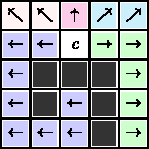
\includegraphics[width=\linewidth]{images/botea-cpd.pdf}
				\caption[Movement information in grid-based CPD.]{Movement-grid for cell $c$ in a grid-based CPD\cite{botea-cpd-2013}.}
				\label{fig:cpd}
			\end{wrapfigure}
			
			The complex part of constructing a CPD is the compression\cite{botea-cpd-2013} of the all-pairs shortest path solution.
			Uncompressed data is usually too large as the space requirement is in $\bigo{n^2}$ or even $\bigo{n^2 \log n}$ for graphs.
			A combination of compression techniques can be used to get sufficient results.
			This includes the encoding of whole areas with the same movement operations, \term*{run-length encoding} (\term*{RLE}) and the use of default values to reduce the number of explicitly stored values\cite{botea-cpd-2013}.
			Compared to uncompressed data, a compression factor of 950 was achieved for a road network.
	
\section{Geometric routing}
\label{sec:geometric-routing}

	Finding paths in a geometric domain, also called the \term{euclidean shortest path} problem, is the process of determining shortest paths without a graph but through open spaces avoiding obstacles.
	There are two main strategies for finding Euclidean shortest paths:
	Generating edges for graph-based routing or creating a shortest paths map, a structure similar to CPDs.
	
	\subsection{Visibility graphs}
	\label{subsec:visibility-graph}
	
		The first mechanism uses a standard graph-based shortest path algorithm, but the edges in the graph are generated using one of multiple possible approaches.
		One approach creates a so-called \term{visibility graph}, which is a normal graph with edges between vertices that are visible to each other.
		Or in other words, for any two $u, v \in V$ an edge $(u, v) \in E$ exists if and only if no obstacle intersects with this edge.
		A visibility graph might become very large, the worst-case regarding the size is a complete graph with $\bigo{|V|^2}$ many edges.
		
		Alternatives to the visibility graph generation are based on Voronoi diagrams or skeletonization methods.
		However, routing results on such graphs are not necessarily optimal\cite{graser-osm-open-spaces}, since a straight edge between visible vertices is the shortest possible connection.
		
		Source and destination locations must be part of the graph and can be connected with the same algorithm used to create the graph itself.
	
	\subsection{Continuous Dijkstra paradigm}
	\label{subsec:continuous-dijkstra}
	
		The second strategy, the \term{continuous Dijkstra paradigm}, creates a map of regions, similar to CPDs, starting from a source vertex $s$.
		Regions are characterized by the fact that all vertices within a region have the same predecessor on the shortest path from $s$.
		Following back the predecessors yields the shortest path from $s$ to a given location.
		This map can also be seen as a tree with root $s$ and each region as a node, which might remind one of Dijkstra's algorithm giving this approach its name\cite{mitchell-discrete-geodesic}.
		
		To precisely determine these regions, so-called \term[wavefront]{wavefronts} propagating through open spaces are used.
		A well-fitting analogy for this approach is the propagation of water waves traveling through a 2D space, folding around obstacles, colliding with each other and finally reaching the destination location.
		Collisions between wavefronts and obstacles as well as collisions between two wavefronts determine the regions' boundaries with the source of the wavefront as its predecessor.
		After detecting such a collision, the angular region of the wavefront is adjusted depending on the type of collision.
		The fundamental difficulty of this approach is the efficient detection and handling of collisions.
		Efficient algorithms are presented in \Cref{subsec:related-work-geometric-routing}.

\section{Agent-based systems and simulations}

	Simulating complex systems with numerous autonomous individuals is difficult, but using so-called \term[agent]{agents} with independent behavior and decision-making breaks down this complexity\cite{macal-introductory-tutorial}.
	Interactions between two agents and between agents and the environment are essential to this.
	
	Modeling agents can be arbitrarily complex because agents make decisions independently without any central controlling unit.
	More sophisticated agents may have a specific goal, can adapt to the environment and thus must be able to memorize and plan things.
	
	Agents usually model humans but can represent non-living things like companies or cars.
	Many simulations use pedestrians (or generally humans) as agents to better understand or utilize human behavior but other scenarios and types of agents are possible as well\cite{macal-introductory-tutorial}.

	Studying pedestrians requires a spatial environment and algorithms finding optimal paths\cite{kneidl-borrmann-hartmann-navigation,gloor-hybrid-pedestrian-routing,teknomo-millonig-routing}.
	This includes \hyperref[sec:graph-routing]{graph-based routing} but may utilize \hyperref[sec:geometric-routing]{geometric routing} as well\cite{kneidl-borrmann-hartmann-navigation}.
	In this thesis, these two concepts are combined to enhance the pathfinding component of agent-based simulations.
	
	\subsection{The MARS framework}
	
		This work aims to enhance agent-based simulations created using the framework \term*{MARS} (Multi-Agent Research and Simulation).
		MARS is a C\#/.NET framework to create and execute agent-based simulations and is developed by the eponymous research group of the Hamburg University of Applied Sciences (HAW) in Hamburg, Germany\footnote{\url{https://www.mars-group.org}}.
		The framework provides components, algorithms and tools to create tick-based simulations with multiple agents, different data layers and numerous static entities populating the environment.
		
		MARS contains several data structures and algorithms specifically for pathfinding, such as a spatial graph and the A* algorithm.
		It also contains numerous spatial indices, mathematical operations and classes to serialize the trajectories of agents.
		 
		This work is based on the MARS framework to be directly usable by simulations and uses the mentioned spatial graph and A* algorithm.
		More details on the design and implementation are given in \Cref{chap:design} and \ref{chap:implementation}.